\documentclass{school-22.101-notes}
\date{December 13, 2011}

\begin{document}
\maketitle

\clearpage
\topic{Gamma Interaction}
GI was not covered Fall 2011. Prof. Yip covered it over two lectures Fall 2012. Basic concepts: 
\begin{enumerate}
\item Gamma rays are electromagnetic radiations produced by nuclear transitions. These are typically \hi{photons with energies in 0.1$\sim$10 MeV}. 

\item The attenuation (either scattering or absorption, any process that removes gamma from the beam) of the intensity of a beam of gamma rays follows a true \hi{exponential} variation with respect to distance $I(x) = I_0 e^{-\mu x}$, unlike that of charged particle penetration. 

\item 3 types of GI: Compton scattering, photoelectric interaction, and pair production. Compton scattering is the most important one. These three process are independent so the total attenuation coefficient (xs) is the sum of the three. The approach is the same for all three: we consider $\frac{\dsigma_X}{\dOmega}, \frac{\dsigma_X}{\dT}$, where $X = C$ for Compton, $\tau$ for photoelectric effect, and $\kappa$ for pair production. 
  \begin{table}[ht]
    \centering
    \begin{tabular}{cccc} \hline
      Target material& Absorption & Elastic Scattering & Inelastic Scattering \\  \hline \hline
      electrons & photoelectric & Thomson & Compton \\  \hline
      nucleus & x & x & x \\ \hline
      electric field around nucleus & pair production & x & x \\ \hline
    \end{tabular}
    \caption{Gamma Interaction Types}
  \end{table}

\end{enumerate}

\subtopic{Compton Scattering}
Compton scattering is the inelastic (photon loses energy) relativistic scattering by a free electron,  
which can be treat similar to neutron scattering, though we have to consider relativistic kinetics. For Compton

\begin{enumerate}
\item Basic relations. We define $E_{\gamma} = \hbar c k, \omega = 2 pi \gamma = ck$, where $c$ is speed of light and $\lambda \gamma = c$. We consider conservation of momentum and conservation of energy to get SY7 Eq.17.5 - 17.8: 
\eqn{ \lambda' - \lambda = \frac{c}{v'} - \frac{c}{v} = \frac{h}{m_e c} ( 1 - \cos \theta) }
\eqn{ \frac{\omega'}{\omega} = \frac{1}{1 + \alpha (1 - \cos \theta)}} 
where $\alpha = \frac{\hbar \omega}{m_e c^2} = \left( \frac{A-1}{A+1} \right)^2$ which characterizes the kinematics, and $\theta$ is scattering angle ($\theta = 0$ means forward scattering, $\theta = \pi$ means ...). 

\item Derivation of $\frac{\dsigma_c}{\dOmega}$ by Klein \& Nishine (1928) using relativistic QM: 
\eqn{ \frac{\dsigma_c}{\dOmega} = \frac{r_e^2}{4} \left( \frac{\omega'}{\omega} \right)^2 \left[ \frac{\omega}{\omega'} + \frac{\omega'}{\omega} - 2 + 4 \cos^2 \theta \right] }
where $\displaystyle r_e = \frac{e^2}{m_p c^2} = 2.83 \times 10^{-13} \cm$ which is the classical radius of the electron. 

\item We make two assumptions: unpolarized radiation (polarized is complex, so we ignore it), and small $\alpha$: 
\begin{enumerate}
\item For unpolarized radiation, we consider the averaging over angle $\phi$, to get SY7 Eq.17.18, 17.19.

\item For small $\alpha$ (low energy limit), Compton becomes Thompson, we can approximate $\omega' \sim \omega$ and arrive at Eq.17.16, 
\eqn{ \boxed{ \left( \frac{\dsigma_c}{\dOmega} \right)_{\mathrm{unpol}} = \frac{r_e^2}{2} (1 + \cos^2 \theta) } }
which implies that scattering is symmetric about $90\degree$. 
\end{enumerate}
Make sure you understand Fig~\ref{17.3} which says that Thompson is symmetric, and as $\alpha \up$ we become forward biased. 
\begin{figure}
  \centering
  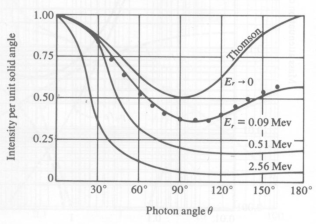
\includegraphics[width=4in]{images/ni/17.3.png}
  \caption{Angular Distribution of Compton Scattering at Various Incident Energies $E_r$. (SY7 Fig. 17.3, Heitler)} \label{17.3}
\end{figure}

\item Energy distribution of Compton electrons and photons: we combine two equations,
  \eqn{ \frac{\dsigma_c}{\dtheta} = \frac{\dsigma_c}{\dOmega} 2 \pi \sin \theta }
  \eqn{ \frac{\dsigma_c}{\domega'} = \frac{\dsigma_c}{\dtheta} \left| \frac{\dtheta}{\domega'} \right| }
  \eqn{ \frac{\dsigma_c}{\dT} = \frac{\dsigma_c}{\domega'} \left| \frac{\domega'}{\dT} \right| = \frac{\dsigma_c}{\domega'} \frac{1}{\hbar} }
where we can use $\hbar \omega' = \hbar \omega - T$. We arrive at Fig.~\ref{17.4}, where notice there is an edge effect (called Compton edge). 

\begin{figure}
  \centering
  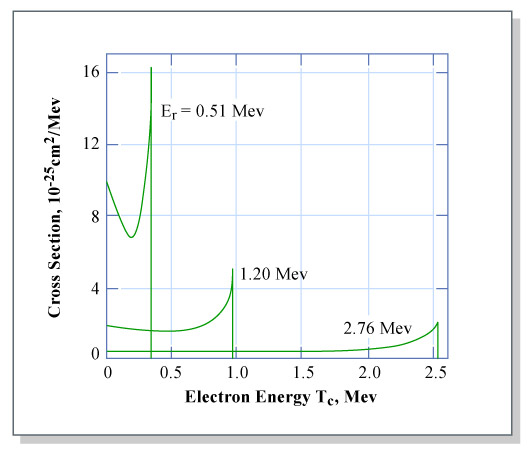
\includegraphics[width=4in]{images/ni/17.4.png}
  \caption{Energy Distribution of Compton Electrons for Several Incident Gamma-ray Energies. (SY7 Fig. 17.4, Meyerhof)} \label{17.4}
\end{figure}
\end{enumerate}


%%%%%%%%%%%%%% 2nd type %%%%%%%%%%%%%%%%
\subtopic{Photoelectric Effect}
\begin{enumerate}
\item Set-up: incoming momentum $\hbar k$ hit an atom and produces an ejected electron (photoelectron) with $p, T$ and an excited recoil atom with $p_a, T_a$. Another way to put it: absorption of an incident gamma ray and the ejection of an atomic electron and the excitation of the recoiling atom. 

\item Conservation equations:
  \eqn{ \hbar k = P + P_a} 
  \eqn{ \hbar \omega = T + T_a + B }
  where $B$ is the binding energy of the atomic electron. Typically $T_a, B$ are small: $B$ is atomic energy which is smaller than nuclear energy, and $T_a$ is small because the mass of this atom is a lot larger than the photoelectron. That is, photoelectron gets most of the energy. 

\item We derive Eq. 18.4, 
\eqn{ \frac{\dsigma_{\tau}}{\dOmega} = 4 \sqrt{2} \frac{r_e^2 Z^5}{(137)^4} \left( \frac{m_e c^2}{\hbar \omega} \right)^{7/2} \frac{\sin^2 \theta \cos^2 \phi}{\left( 1 - \frac{v}{c} \cos \theta \right)^4} }
Key points: the important factor is really $(\vec{p} \dot \vec{\epsilon})^2$. 
\begin{enumerate}
\item Photoelectri effect is not isotropic and not azimuthally symmetric. 
\item $Z$ is just the number of scatters. $Z^2$ means Coulomb effect, for instance. $Z^5$ means the interaction is complicated, and that it is characteristic of atoms with high-$Z$. 
\end{enumerate}

\item We integrate the differential xs over all solid angles to get the total xs: 
  \eqn{ \sigma_{\tau} = 4 \sqrt{2} \sigma^0 \frac{Z^5}{(137)^4} \left( \frac{m_e c^2}{\hbar \omega} \right)^{7/2} }
  In practice, we get $\sigma_{\tau} \propto \frac{Z^n}{(\hbar \omega)^3}$ where $n = 4 \sim 4.6$ due to screening effect. 

\item Plot $\sigma_{\tau}$ vs. $\hbar \omega$ in Fig.~\ref{GI}: in low energy range we expect photoelectric effect to dominate. Since $Z$ comes in at high power, the photoelectrical effect is more obvious for high-$Z$ isotopes. This is why we use lead instead of Al to take out gamma rays. 
  \begin{figure}[ht]
    \centering
    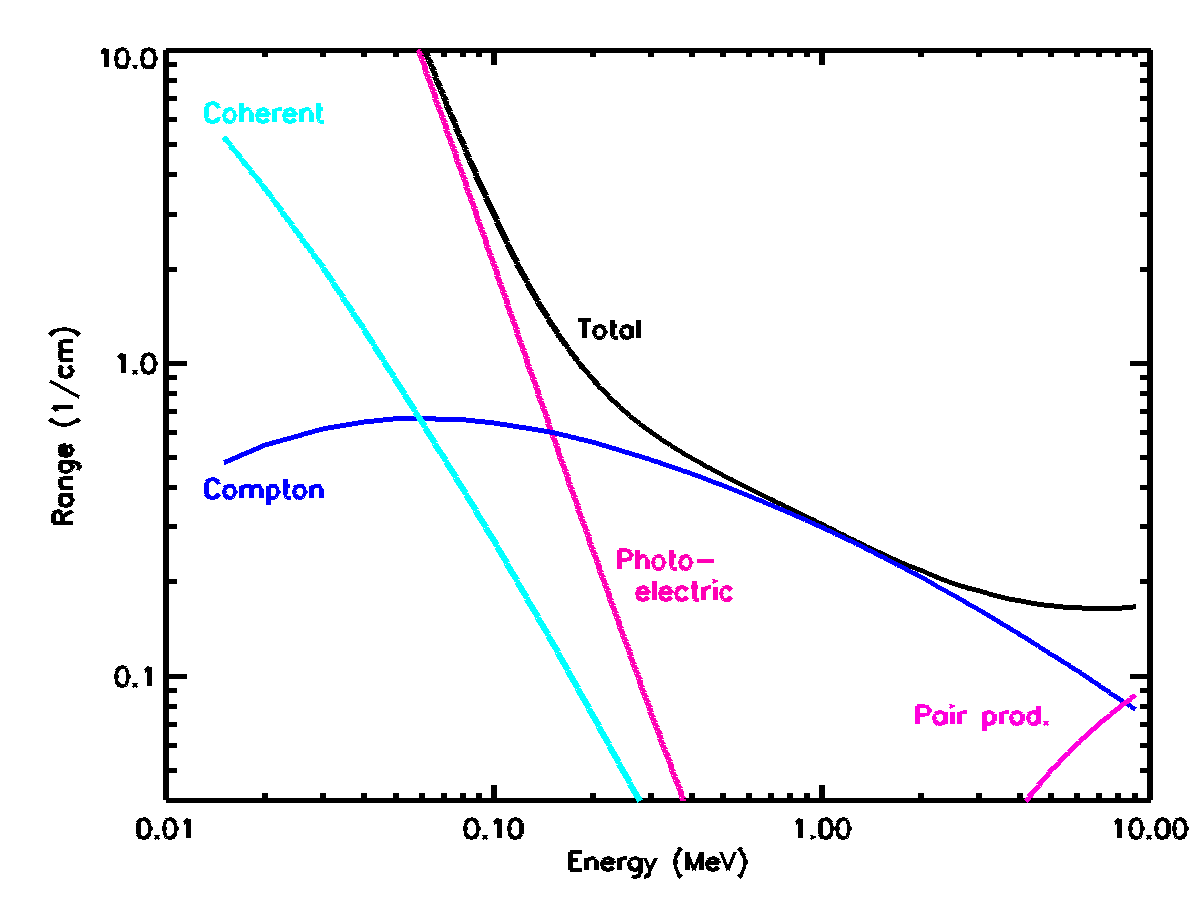
\includegraphics[width=4in]{images/ni/GI.png}
    \caption{Cross section vs. Energy for Three Gamma Interaction} \label{GI} 
  \end{figure}
\end{enumerate}


%%%%%%%%%%%%%% 3rd type %%%%%%%%%%%%%%%%
\subtopic{Pair Production}
\begin{enumerate}
\item Set-up: gamm ray with $\hbar \omega$ ($\hbar \omega > 1.02$ MeV) hits an atom, generate a positron $e^+$ (or written as $\beta^+$) with $p_+, T_+$, and an electron $\beta$ with $p, T_-$. The two would generate annihilation radiation. 

\item Again we start with conservation equations: 
\eqn{ \hbar \vec{k} = \vec{p}_+ + \vec{p} }
\eqn{ \hbar \omega = (T_+ + m_c c^2) + (T_- + m_e c^2) }

\item We arrive at the differential xs in Eq. 18.10, 18.11 and Fig.~\ref{18.8}. 
  \begin{figure}[ht]
    \centering
    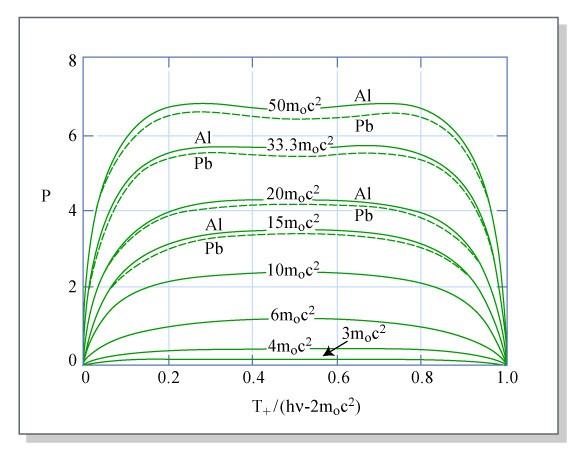
\includegraphics[width=4in]{images/ni/18.8.png}
    \caption{Calculated Energy Distribution of Positron Emitted in Pair Production} \label{18.8} 
  \end{figure}

\item Integrate to get the total xs: Eq.18.12, 18.13 (one without screening one with complete screening). 

\end{enumerate}




%%%%%%%%%%%%%% Together %%%%%%%%%%%%%%%%
\subtopic{Mass Attenuation}
We piece the three effects together to get the mass attenuation, $\mu = \mu_C + \mu_{\tau} + \mu_{\kappa}$, and 
\eqn{ \frac{\mu}{\rho} \sim \left( \frac{N_0}{A} \right) \begin{dcases*} Z \sigma_C & $\sigma_C \sim \frac{1}{\hbar \omega}$, per electron \\
 \sigma_{\tau} & $\sigma_{\tau} \sim \frac{Z^5}{\left( \hbar \omega \right)^{7/2}}$, per atom \\
\sigma_{\kappa} & $\sigma_{\kappa} \sim Z^2 \ln \left( \frac{2 \hbar \omega}{m_e c^2} \right)$, per atom 
\end{dcases*} }
Fig.~\ref{18.13} is a smily face: less than 1 MeV Compton scattering dominates and decreases as gamma ray energy increases; around 1 MeV the attenuation is about constant due to photoelectric effect; between 1 MeV and 5 MeV the attenuation increase with respect to energy due to pair production. 

  \begin{figure}[ht]
    \centering
    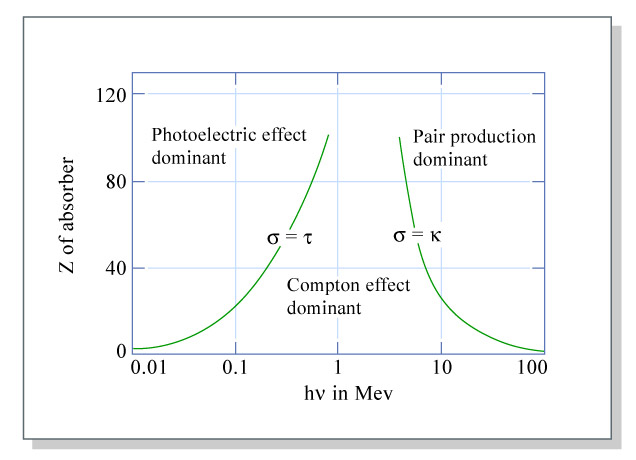
\includegraphics[width=4in]{images/ni/18.10.png}
    \caption{} \label{18.10} 
  \end{figure}

  \begin{figure}[ht]
    \centering
    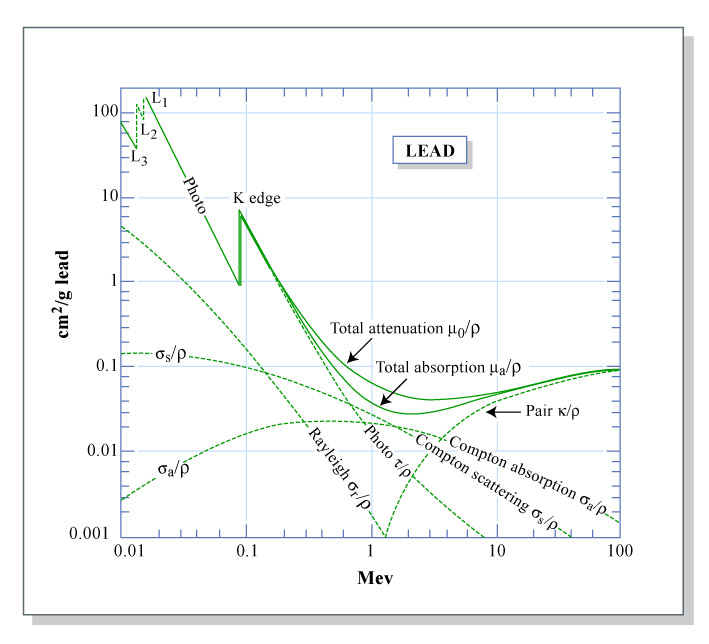
\includegraphics[width=4in]{images/ni/18.13.png}
    \caption{Mass Attenuation Coefficients for Photons in Lead} \label{18.13} 
  \end{figure}


\subtopic{Pulse Height Spectra, Radiation Detection}
Mostly we detect electrons; we want to collect charge flow (current); the larger the current, the larger the pulse height, which is proportional to the energy the gamma rays bring in $\propto \hbar \omega$.

We consider using NaI detector to detect 1.37/2.75 MeV gamma ray into \ce{^{24}Na}. 

  \begin{figure}[ht]
    \centering
    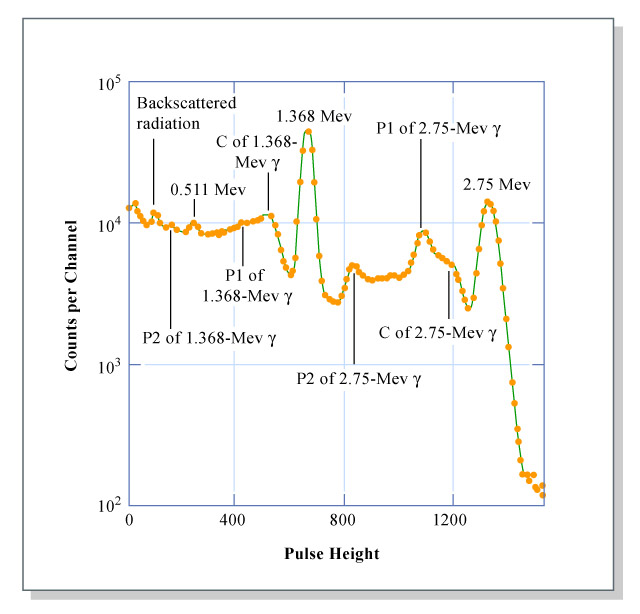
\includegraphics[width=0.49\textwidth]{images/ni/19.1.png} 
    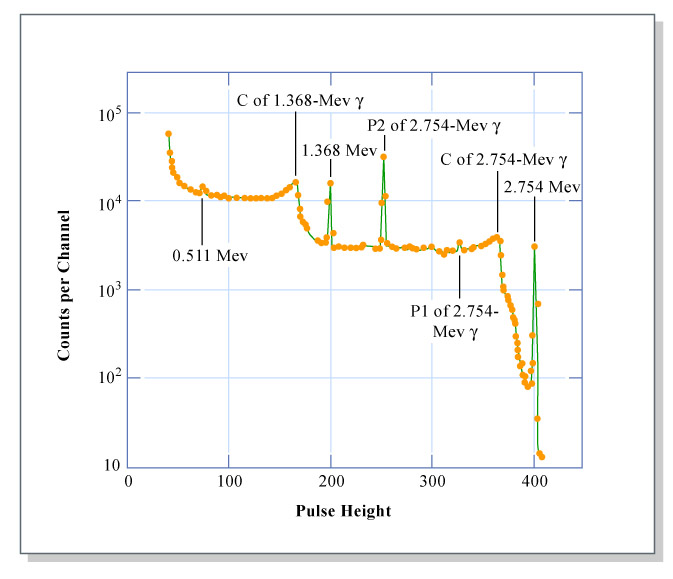
\includegraphics[width=0.49\textwidth]{images/ni/19.2.png} 
    \caption{Pulse Height Spectra Obtained Using a Na-I, Li-Ge Detector} \label{19.1} 
  \end{figure}

Interpretation of Fig.~\ref{19.1}:
\begin{itemize}
\item Compton: peak at 2.75 MeV and the decrease afterwards.
\item Compton edge: the 2.5 MeV between the `C of 2.75 MeV' and the `2.75 MeV' peak. 
\item Anniliation: the 0.511 MeV between P1 and 2.75 MeV peak, and the 0.511 MeV between P1 and P2. P1 $>$ P2, where P1 is the probability that one escapes, and P2 is the probability that two escape. 
\end{itemize}

Interpretation of Fig.~\ref{19.2}: we get the same shape, except P2 $>$ P1. The explaination is, if we let P to be the probability of escape, the P1 $=$ 2 P (1-P), P2 = P$^2$. Thus if $P \ll 1, P1 > P2$, and when $P\sim 1, P2 > P1$. 

\end{document}
